\documentclass[10pt]{beamer}
\usetheme{Boadilla}
\usecolortheme{seahorse}
\usepackage{amssymb,amsmath}
\usepackage[utf8]{inputenc}

\usepackage{xcolor}
\usepackage{hyperref}
\usepackage{multicol}



% beamer style 

\definecolor{xoveticblue}{HTML}{3cafc2} % UBC Blue (primary)
\definecolor{xoveticorange}{HTML}{e58923}
\definecolor{xoveticdarkorange}{HTML}{d97b27}
\hypersetup{
    colorlinks = true,
    linkcolor = xoveticblue,
    urlcolor = xoveticblue
}


\setbeamercolor{palette primary}{bg=xoveticorange,fg=white}
\setbeamercolor{palette secondary}{bg=xoveticblue,fg=white}
\setbeamercolor{palette tertiary}{bg=xoveticdarkorange, fg=white}
\setbeamercolor{palette quaternary}{bg=xoveticorange, fg=white}
\setbeamercolor{structure}{fg=xoveticorange} % itemize, enumerate, etc
\setbeamercolor{section in toc}{fg=xoveticorange} % TOC sections
\setbeamercolor{subsection in head/foot}{bg=xoveticorange,fg=white}



\usepackage[capitalise, noabbrev, nameinlink]{cleveref}
\usepackage{float}
\usepackage{booktabs}
\usepackage{makecell}
\setbeamertemplate{caption}[numbered]

% -------- Portada ---------
\title[\textcolor{white}{Automatic covariates selection in DRM}]{Automatic covariates selection in dynamic regression models with application to COVID-19 evolution}

\author[Ana Ezquerro, Germán Aneiros, Manuel Oviedo]{
    Ana Ezquerro \inst{1} 
    \and 
    Germán Aneiros \inst{2}
    \and 
    Manuel Oviedo \inst{3}
}
\institute[]{
   \inst{1} University of A Coruña, \texttt{ana.ezquerro@udc.es}
\and
    \inst{2} CITIC, Grupo MODES, Departamento de Matemáticas, University of A Coruña, \\ \texttt{german.aneiros@udc.es}
\and
    \inst{3} CITIC, Grupo MODES, Departamento de Matemáticas, University of A Coruña \\ \texttt{manuel.oviedo@udc.es}
}

\date{Congreso XoveTIC 2022}

\begin{document}

\frame{\titlepage}

\begin{frame}
    \frametitle{Introduction}
        The \textbf{linear dynamic regression model} defines the linear dependence between a stochastic process $Y_t$ and a set of processes $\mathcal{X} =  \{ X_t^{(1)}, ..., X_t^{(m)} \}$:

        \[  Y_t = \beta_0 + \beta_1 X_{t-r_1}^{(1)} + \cdots \beta_m X_{t-r_m}^{(m)} + \eta_t
        \]

        constrained to $r_i\geq 0$ for $i=1,...,m$ and $\eta_t \sim \text{ARMA}(p,q)$\footnote{here we denote the AutoRegressive Moving Average model as ARMA.}.



        \begin{itemize}
            \item \cite{cryer2008time} proposed the \textit{prewhitening} as a technique for removing spurious correlation between processes in order to detect linear correlation.
            \item We propose a forward-selection method that iteratively adds regressor variables (from a set of candidates) $Y_t$ is \textit{significantly} dependent with.
            \item Widespread application in financial, economic, political and biomedical fields.
            \item \textbf{Procedure}: analyze the mutual impact of several variables in order to define mathematical relationships and use them in forecasting.
        \end{itemize}

\end{frame}

\begin{frame}{Prewhitening}

    \cite{cryer2008time} states that if a linear correlation between two processes $X_t$ and $Y_t$ exists for some $k\leq 0$ then
    
    \[ \rho_k(\ddot{X}_t, \ddot{Y}_t) \qquad \text{is statistically significant,} \] 

    \begin{itemize}
        \item $\rho_k(X_t^{(1)}, X_t^{(2)})$ is the cross-correlation function between processes $X_t^{(1)}$ and $X_t^{(2)}$ lagged $k$ moments.
        \item $\ddot{X_t}$ and $\ddot{Y}_t$ are obtained via some linear filter application to $X_t$ and $Y_t$, respectively, ensuring one of them is white noise and the other is a stationary process (\textit{prewhitening}).
    \end{itemize}

    \begin{block}{Our proposal}
        \vspace{0.2em}
        \begin{itemize}
            \item Iteratively adds in the model significant covariates with their respective lags that optimize some information criterion (IC) of the resultant residuals.
            \item Uses the \textbf{residuals} of the last model created (by adding covariates) to check the existence of correlation between the dependent variable and a \textbf{new covariate candidate}.
        \end{itemize}
    \end{block}

\end{frame}

\begin{frame}{Example of spurious correlation and prewhitening}
    \begin{figure}
        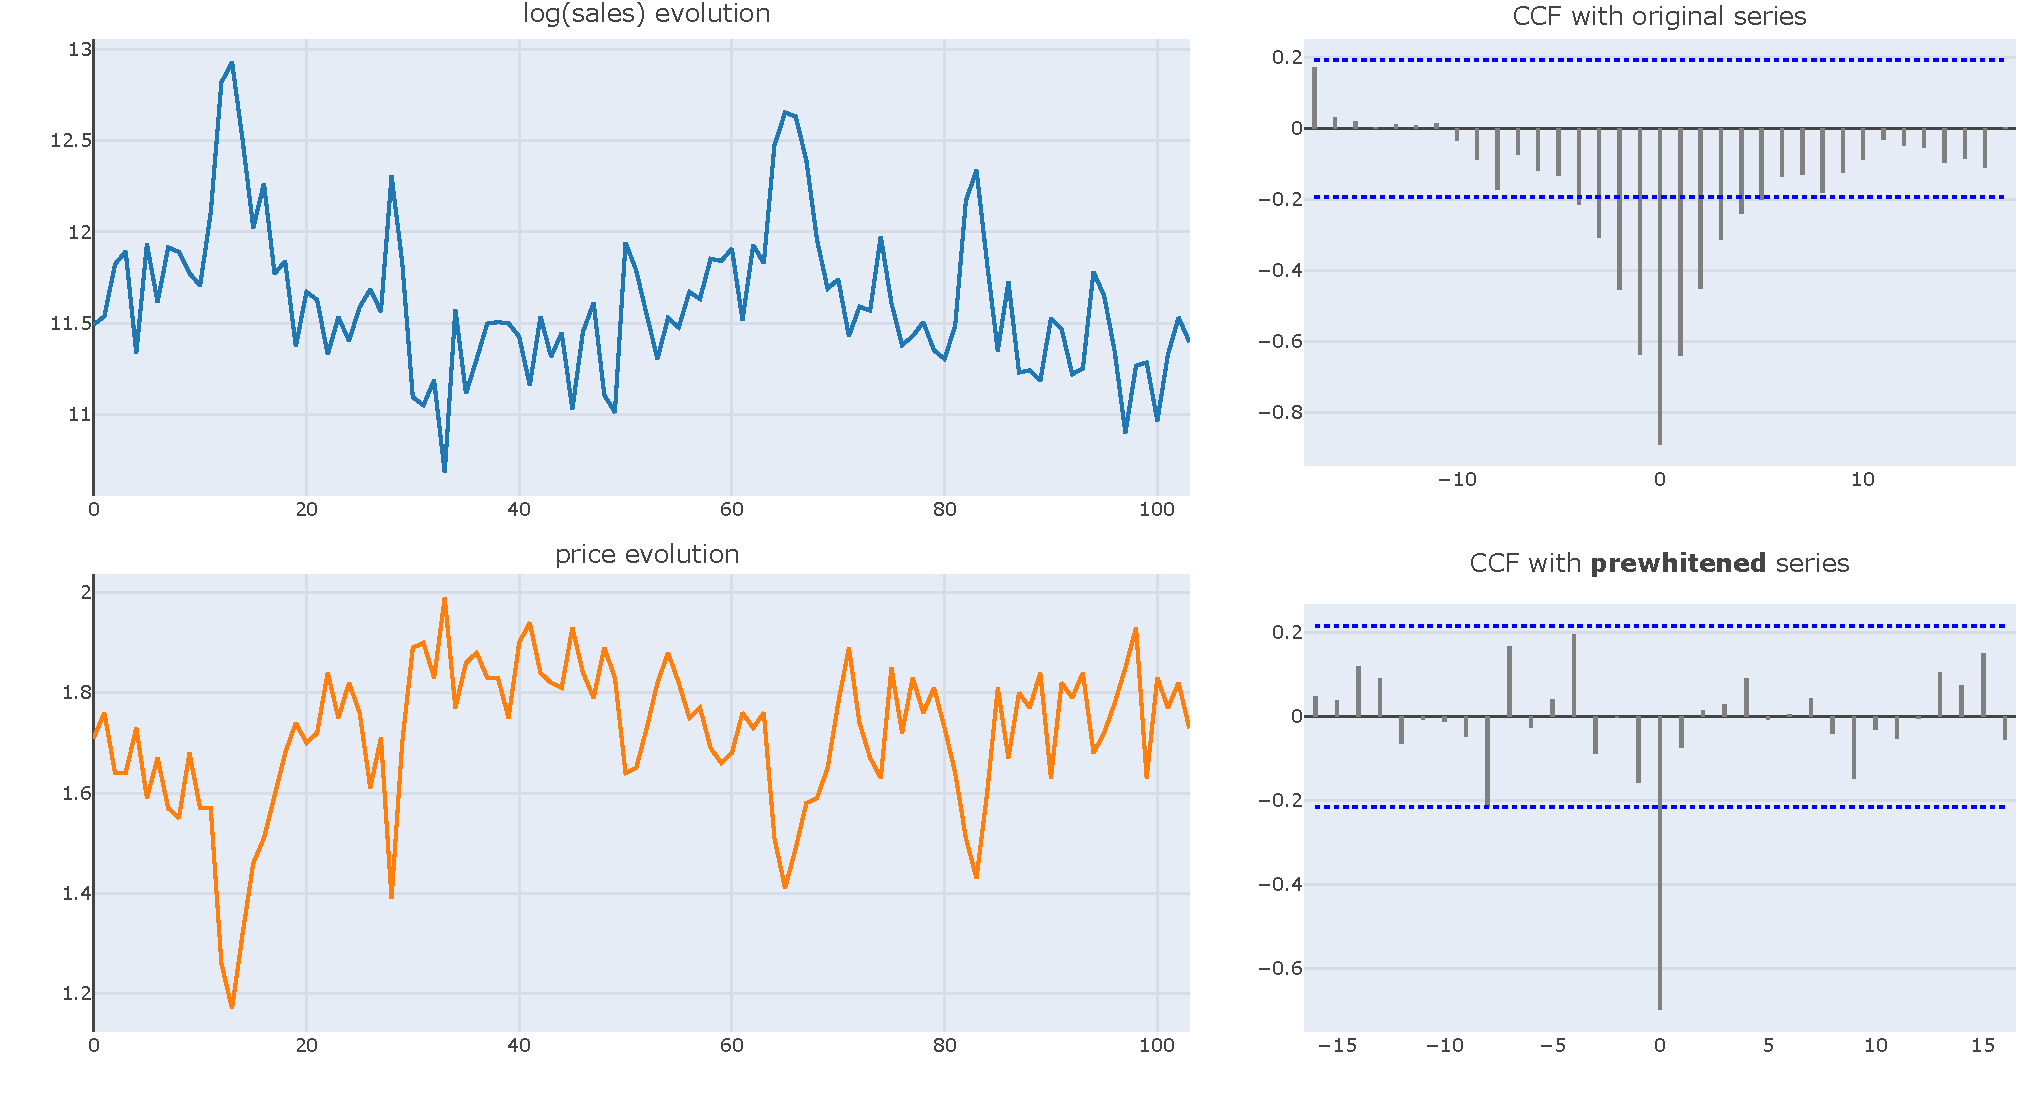
\includegraphics[scale=0.35]{example prewhitening.pdf}
    \end{figure}
    
\end{frame}

\begin{frame}{Methodology}
    

    Let $Y_t$ be the dependent variable and $\mathcal{X}$ the set of covariates candidates. Thus, selection proceeds as follows:
    
    \begin{enumerate}
        \item Initialization. Consider $X_t^\text{best}$ as the covariate (lagged $r$ moments) that minimizes the IC of the constructed model with $Y_t$:
        \[ X_t^\text{best} = \underset{X_t\in\mathcal{X}}{\arg\min} \Bigg\{ \text{IC}\Bigg( Y_t = \beta_0 + \beta_1 X_{t-r}^\text{best} + \eta_t \Bigg)\Bigg\} \] 
        \item Iteration. Use the regression errors ($\eta_t$) of the last model created to check if some correlation exists between the rest of the covariates not yet added to the model. Find again the ``best'' variable and add it to the model to obtain a new IC value. If this value improves the last one achieved, repeat this step. If it does not, stop the iteration.
        \item Finalization. The errors of the last fitted model must satisfy the stationary property. In other case, consider the regular differentiation of all data and start again the procedure.
    \end{enumerate}
\end{frame}

\begin{frame}{Example of the iterative selection step by step}


    \begin{table}
        \centering\small
        \setlength{\tabcolsep}{5pt}
        \caption{From \href{https://www.worldometers.info/coronavirus/}{worldmeters} source, model the evolution of \textit{exitus} cases in Spain due to the COVID-19 considering other country data} 
        \label{covid19}
    
        \begin{tabular}{|l|ccc|}
            \hline
            \textbf{Covariate}           & \textbf{Lag}  & \textbf{Coefficient est. (s.e)} & \textbf{AICc}          \\ 
            \hline 
            \texttt{confirmed\_spain}    & 0             & 0.0064 (0.0009)                 & 5596.641             \\ 
            \texttt{recovered\_portugal} & -1            & -0.0337 (0.0063)                & 5550.963             \\
            \texttt{recovered\_france}   & 0             & 0.0646 (0.0142)                 & 5540.655             \\
            \texttt{confirmed\_france}   & 0             & -0.0033 (0.0007)                & 5522.699             \\
            \texttt{confirmed\_portugal} & -13           & 0.0395 (0.0085)                 & 5504.169             \\
            \texttt{recovered\_spain}    & -7            & -0.0669 (0.0176)                & 5500.573             \\ 
            \hline 
        \end{tabular}
    \end{table}    
    \begin{itemize}
        \item \textbf{Note}: This model was fitted with differentiated data.
        \item \texttt{deaths\_england}, \texttt{deaths\_france}, \texttt{confirmed\_england}, \texttt{recovered\_england} and \texttt{deaths\_portugal} were not included in the model.
        \item The residuals of the model follow an ARMA$(1,1)\times (1,1)_7$ with parameters:
        \[
        \begin{array}{l}
            \phi_1=0.9724 (0.0131), \ \theta_1=-0.7508 (0.0370), \\
            \Phi_1=0.6958 (0.1892), \ \Theta_1=-0.5512 (0.2215)
        \end{array}
        \] 
    \end{itemize}
\end{frame}

\begin{frame}{Simulation procedure}
    \begin{enumerate}
        \item Seven time series (modelable by an ARIMA) were generated: six act as covariate candidates $\mathcal{X}=\{X_t^{(1)}, ..., X_t^{(6)}\}$ with random lags $r\in[0, 6]$, and the remaining as the errors of the model.
        \item Formally, each simulation follows this scheme:
        \[ Y_t = \beta_0 + \beta_1 X_{t-r_1}^{(1)} + \beta_2 X_{t-r_2}^{(2)} + \beta X_{t-r_3}^{(3)} + \eta_t \] 
        where $\eta_t\sim\text{ARMA}(p,q)$, $\beta_0,...,\beta_3$ are randomly generated and $r_i\in[0,6] $ for $i=1,..,3$.
        \item Selection method was tested with different configurations:
        \begin{itemize}
            \item Changing the IC with three different options: AIC, BIC or AICc.
            \item Changing the method to check stationary: via the Dickey-Fuller test or via adjusting an ARIMA and checking the differentiation order.
        \end{itemize}
    \end{enumerate}
    
\end{frame}

\begin{frame}{Example of one simulation result}
    \begin{figure}
        \caption{Code output when launching the function \texttt{auto.fit.arima.regression()} that implements our approach}
        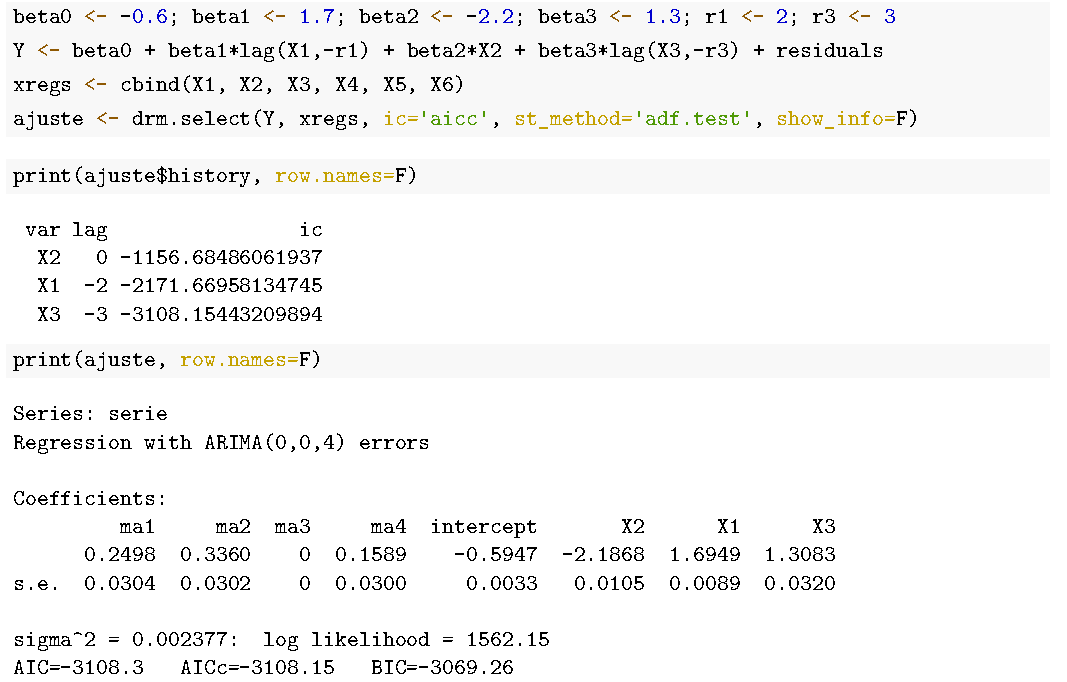
\includegraphics[scale=0.5]{simulation-example.pdf}
    \end{figure}
    
\end{frame}


\begin{frame}{Results of multiple simulations where $\eta_t\sim\text{ARMA(p,q)}$}

    \begin{table}
        \centering\small 
        \renewcommand{\arraystretch}{1.3}
        \setlength{\tabcolsep}{10pt}
        \label{simulations1}
        \caption{Percentage of covariates correctly added to the model}
        \begin{tabular}{|c|ccc|ccc|}
            \cline{2-7}
            \multicolumn{1}{c|}{}   & \textbf{AIC}  & \textbf{BIC}  & \textbf{AICc}            & \textbf{AIC}      & \textbf{BIC}   & \textbf{AICc} \\
            \hline       
            \textbf{adf.test}       & 97.66\%       & 97.66\%        & 97.66\%                 & 3.66\%            & 1.33\%         & 3.66\%        \\
            \textbf{auto.arima}     & 98.33\%       & 98.33\%        & 98.33\%                 & 3.66\%            & 1.33\%         & 3.66\%        \\
            \hline
            \multicolumn{1}{|c|}{}   & \multicolumn{3}{c|}{correctly added (TP)}               & \multicolumn{3}{c|}{incorrectly added (FP)}         \\
            \hline 
            \multicolumn{7}{c}{}                                                                                                                    \\
            \cline{2-7}
            \multicolumn{1}{c|}{}   & \textbf{AIC}  & \textbf{BIC}  & \textbf{AICc}           & \textbf{AIC}      & \textbf{BIC}   & \textbf{AICc}  \\ 
            \hline        
            \textbf{adf.test}       & 96.33\%       & 98.66\%        & 96.33\%                & 2.33\%            & 2.33\%         & 2.33\%         \\
            \textbf{auto.arima}     & 96.33\%       & 98.66\%        & 96.33\%                & 1.66\%            & 1.66\%         & 1.66\%         \\
            \hline 
            \multicolumn{1}{|c|}{}   & \multicolumn{3}{c|}{correctly \textbf{not} added (TN)} & \multicolumn{3}{c|}{incorrectly \textbf{not} added (FN)}  \\
            \hline
        \end{tabular}
    \end{table}

    
    
\end{frame}

\begin{frame}{Results of multiple simulations where $\eta_t\sim\text{ARIMA(p,d,q)}$}
    \begin{table}
        \centering\small 
        \renewcommand{\arraystretch}{1.3}
        \setlength{\tabcolsep}{10pt}
        \label{simulations2}
        \caption{Percentage data about the performance of the selection method}
        \begin{tabular}{|c|ccc|ccc|}
            \cline{2-7}
            \multicolumn{1}{c|}{}   & \textbf{AIC}  & \textbf{BIC}  & \textbf{AICc}            & \textbf{AIC}      & \textbf{BIC}   & \textbf{AICc} \\
            \hline       
            \textbf{adf.test}       & 93.33\%       & 93.33\%        & 93.33\%                 & 4.33\%            & 0.30\%         & 4.33\%        \\
            \textbf{auto.arima}     & 94.33\%       & 94.66\%        & 95.33\%                 & 5.00\%            & 1.33\%         & 5.00\%        \\
            \hline
            \multicolumn{1}{|c|}{}   & \multicolumn{3}{c|}{correctly added (TP)}               & \multicolumn{3}{c|}{incorrectly added (FP)}         \\
            \hline 
            \multicolumn{7}{c}{}                                                                                                                    \\
            \cline{2-7}
            \multicolumn{1}{c|}{}   & \textbf{AIC}  & \textbf{BIC}  & \textbf{AICc}           & \textbf{AIC}      & \textbf{BIC}   & \textbf{AICc}  \\ 
            \hline        
            \textbf{adf.test}       & 95.00\%       & 98.66\%        & 95.00\%                & 6.66\%            & 6.66\%         & 6.66\%         \\
            \textbf{auto.arima}     & 94.66\%       & 99.66\%        & 95.66\%                & 4.66\%            & 5.33\%         & 4.66\%         \\
            \hline 
            \multicolumn{1}{|c|}{}   & \multicolumn{3}{c|}{correctly \textbf{not} added (TN)} & \multicolumn{3}{c|}{incorrectly \textbf{not} added (FN)}  \\
            \hline
        \end{tabular}
    \end{table}
\end{frame}


\begin{frame}{Application to COVID19 evolution}
    \begin{table}
        \centering
        \setlength{\tabcolsep}{10pt}
        \caption{Information about the dynamic regression model constructed via selection of multiple vaccination variables to model COVID19 evolution} 
        \label{covid19model}
    
        \vspace{0.5em}
        \begin{tabular}{|l|cc|}
            \hline
            \textbf{Covariate}  & \textbf{Lag}  & \textbf{Coefficient est. (s.e)} \\ 
            \hline 
            \texttt{vac4565}    & -3            & -0.0410 (0.0057)                      \\ 
            \texttt{vac6580}    & -2            & -0.0468 (0.0120)                      \\
            \texttt{vac1845}    & -6            & -0.0901 (0.0047)                      \\
            \hline
            \texttt{vac1218}    & \multicolumn{2}{c|}{Not included in the model} \\
            \texttt{vac80}      & \multicolumn{2}{c|}{Not included in the model} \\
            \hline
            residuals           & ARIMA(4, 0, 0) & \makecell[c]{$\phi_1=2.0816 (0.0810)$ \\ $\phi_2=-1.2837 (0.1152)$ \\ $\phi_4=0.1919 (0.0432)$ } \\
            \hline
        \end{tabular}
    \end{table}    
    \begin{itemize}\small
        \item There is a lagged negative correlation between the vaccination data and COVID-19 evolution.
        \item The vaccination of the young population (from 18 up to 45 years old) has a greater impact in the COVID19 evolution.
        \item The vaccination of the population older than 80 years has no significative impact in the COVID19 confirmed cases.
    \end{itemize}
    
\end{frame}

\begin{frame}{Study on vaccination data aggregated by group of ages}


    \begin{figure}\small
        \caption{Forecasting applied to the dynamic regression model constructed in \ref*{covid19model}}
        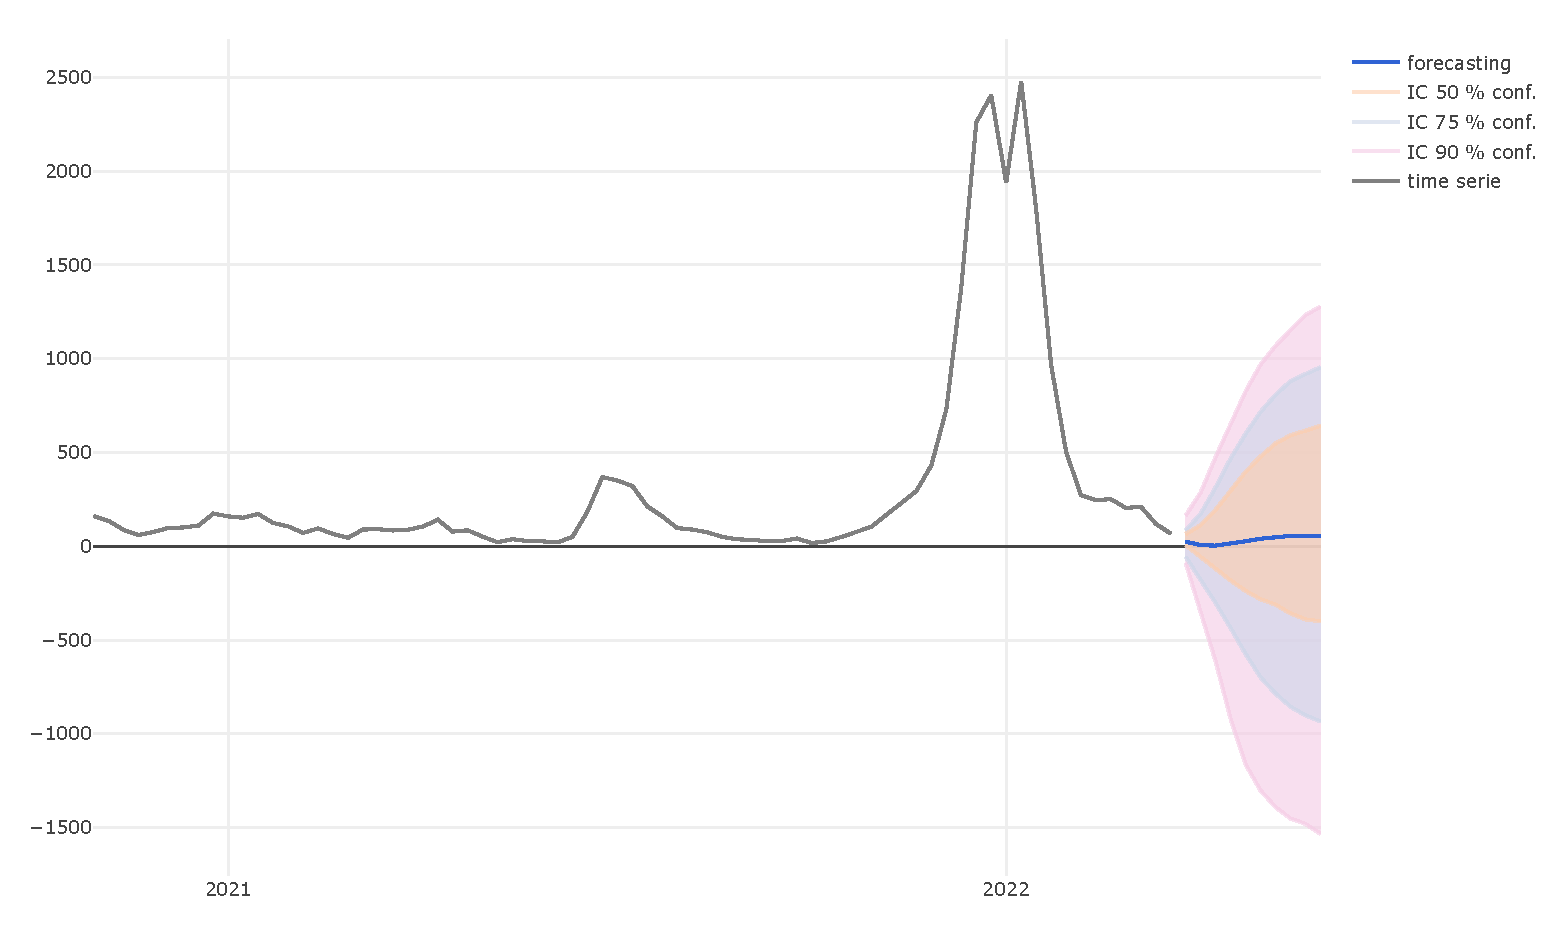
\includegraphics[scale=0.4]{covid19-forecasting.pdf}
    \end{figure}
\end{frame}


\begin{frame}
    \bibliography{bibliography}
    \bibliographystyle{apalike}
\end{frame}

\end{document}  